\chapter{Mercado e competidores} 

Toda empresa competindo em uma indústria tem sua estratégia competitiva,
seja ela explícita ou implícita.   Esta estratégia pode ter sido desenvolvida
explicitamente através de um processo de planejamento ou então evoluiu
implicitamente através de atividades de vários departamentos funcionais da
empresa.   Ao deixar por conta própria, cada departamento funcional irá 
inevitavelmente buscar abordagens ditadas pela orientação dos profissionais
e pelo incentivo dos que estão no comando.

Essencialmente, o desenvolvimento de uma estratégia competitiva é o
desenvolvimento de uma fórmula ampla de como o negócio deverá competir,
quais serão seus objetivos e quais politicas adotar para atingir os objetivos.
A figura \ref{estrategia} ilustra que a estratégia competitiva é a combinação
dos \textit{fins} (objetivos) que a empresa persegue e os \textit{meios}
(políticas) que ela segue para atingí-los \cite{slack2009operations}.  

\begin{figure}[!h]
	\begin{center}
		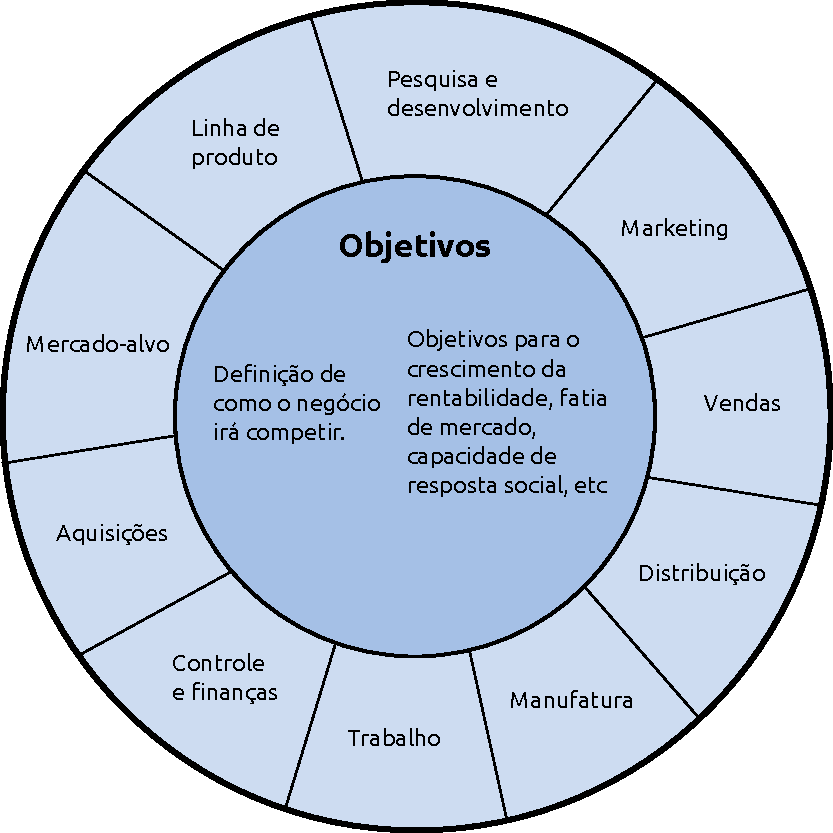
\includegraphics[scale=0.65]{../slides/imagens/estrategia.pdf}
	\end{center}
	\caption{\label{estrategia} A roda da estratégia competitiva.}
\end{figure}
